\chapter{Literature Review}
\label{ch:lit}
\section{Introduction}
In the past decade, conversational chatbots have seen a surge in popularity. Virtual assistants, such as Google Assistant and Amazon Alexa, are now entering our homes via commercially-available Internet of Things devices. In 2017, Google Assistant was present on over 400 million devices \cite{chandra2018}. Furthermore, specialized chatbots have seen an influx within banking, retail, and healthcare \cite{gvr2017}; chatbots represent a trend towards using natural language in the realm of human-computer interaction (HCI).  This literature review will explore how chatbots are implemented, their benefits, and how this project can implement current technologies to create a novel chatbot application.

\section{Chatbots}
When discussing chatbots, their inception is usually cited as Alan Turing’s revered 1950 article `Computing Machinery and Intelligence' \cite{turing1950computing}, wherein Turing considers the question `Can machines think?'. He proposes a scenario called `The Imitation Game' to determine whether a human evaluator can distinguish between a human and a machine during a natural language conversation. This evolved into what we know as the Turing test, which is used to evaluate how effectively a system can imitate human conversation. The goal of most chatbots is not to create true artificial intelligence, but rather to using pattern matching and conversational responses to mimic the responses of a human.

One of the first programs to attempt the Turing test was ELIZA, created by Joseph Weizenbaum between 1964 and 1966 \cite{weizenbaum1976computer}. ELIZA consists of a language analyser and a set of rules by which the `chatterbot' follows. ELIZA used a script called DOCTOR was designed to simulate responses of a psychotherapist during a psychiatric interview – predominantly achieved by the therapist mirroring the responses of the patient  \cite{weizenbaum1976computer}. Although ELIZA may be considered rudimentary and narrow by today’s standards, it forms the basis of our understanding of chatbots and human-computer interaction, and how we can teach machines to mimic human characteristics in dialogue.

Another notable development in chatbots is ALICE (Artificial Linguistic Internet Computer Entity), originally implemented in 1995 by Richard Wallace \cite{wallace2009anatomy}. The system won the Loebner Prize three times, a competition inspired by the Turing Test to judge how well a machine can mimic human responses \cite{keedwell2014loebner}. Although the prize itself was met with some criticism -- Shieber critiques that the goal of the Turing Test is lost on the competition \cite{shieber1994lessons} -- ALICE provides a framework for many of the fundamentals we see in modern chatbots and artificial intelligence.

Intelligent virtual assistants (IVA) are conversation agents that allow users to interact with services and Internet of Things (IoT) devices \cite{chung2018intelligent}. IVAs are ubiquitous in modern life, with most smartphones pre-equipped with a virtual assistant such as Google Assistant or Apple Siri. In many ways, IVAs incorporate many functions of chatbots, as well as providing additional features such as voice input and communication with IoT “smart devices”. IVAs could be seen as a 'superset' of chatbots, and integrate many additional functions and features. Although implementing a virtual assistant is beyond the scope of this project, they represent a concrete example of how effective and abundant dialogue systems currently are.

Industries are seeing a growing trend in chatbot integration in business use. For example, Autodesk integrated IBM’s Watson Assistant \cite{ibm2017watson} to process 100,000 user support conversations, reducing the resolution time of enquiries from 38 hours to 5.4 minutes \cite{ibm2017autodesk}. Many technology companies offer AI cloud services, several of which allow the integration of chatbots including Watson Assistant and Microsoft Azure Bot Service \cite{microsoft2019azure}. The next section will explore and discuss techniques for implementing chatbots and the technologies that can be used.

\newpage
\section{Chatbot Models}
A chatbot usually consists of three key components – natural language processing (NLP), response generation (RG) and a knowledge base \cite{cahn2017chatbot}. Generating a response given the context of a conversation is one of the fundamentals of a chatbot system. These models are usually rule-based or learning-based \cite{wang2013dataset}, and each has its advantages and challenges which will be explored in this section.

\subsection{Pattern Matching}
A rule-based model uses pre-defined patterns in order to match an input to a response. This is seen in ALICE, which uses AIML to construct stimulus-response pairs \cite{wallace2009anatomy}. AIML is an XML-based dialect, which defines units of conversation as a category, with a defined input or stimulus known as a pattern. The response is defined within a template \cite{wallace2009anatomy}, and can make use of utilities such as wildcards and states to help the interpreter to perform some logical processing. Defining patterns is relatively succinct, as shown in Figure~\ref{fig:aiml}, which makes developing a simple question-answer chatbot a somewhat straightforward task.

A rule-based model is inherently limited by the definitions of its ruleset, but they can be effective in closed-domain systems where the context of the conversation is known. This method is easier to implement and debug than other models, but may be thrown by unexpected inputs do not match the definitions of the rules \cite{cahn2017chatbot}. Rule-based models, in particular AIML, are widely-adopted by chatbot platforms such as Pandorabots \cite{pandorabots2019about}.

\begin{figure}[h]
	\begin{lstlisting}
		<?xml version="1.0" encoding="UTF-8"?>
		<aiml version="2.0">
			<category>
				<pattern>HELLO ^</pattern>
				<template>
					<random> <!-- Randomly selected response -->
						<li> Hello! </li>
						<li> Hi there </li>
						<li> Hi, how can I help? </li>
					</random>
				</template>
			</category>
		</aiml>
	\end{lstlisting}
	\caption{A simple AIML pattern}
	\label{fig:aiml}
\end{figure}

\subsection{Neural Networks}
When dealing with open-domain conversations, we can use neural networks to train a chatbot model to deal with unexpected inputs and complex multi-step conversations \cite{vinyals2015neural}. Vinyals et al. use the {\it seq2seq} framework \cite{sutskever2014sequence}, which is based on recurrent neural networks (RNN), to produce a generative conversational model. The advantage of using an RNN is its re-usability for multiple datasets, as well as its efficiency extracting knowledge from noisy datasets, as concluded in \cite{vinyals2015neural}.

Recurrent neural network based models are the simplest and most efficient model to use in neural network language models \cite{mikolov2010recurrent}. Many developments in neural network language models are derivatives of the recurrent neural network language model (RNN LM) defined by \citet{mikolov2010recurrent}. One of the most prominent RNN model is the Tensorflow framework, which trains a deep long short-term memory (LSTM) recurrent neural network \cite{abadi2016tensorflow} for machine learning applications. Tensorflow models have been used widely in research and industry, and implementations have been shown to be notably effective in language and translation tasks \cite{wu2016google}.

The neural network approach has a clear advantage in open-domain conversations and training from multiple datasets, however the results can be unexpected and can require rigorous debugging \cite{pascanu2013difficulty}. Therefore a neural network approach may be outside the scope of this project, although it provides an interesting insight into how language models are being applied in contemporary machine learning systems. 

\newpage
\section{Datasets}
Typically, chatbots are categorised into two groups -- open-domain and closed-domain systems \cite{ilievski2018building}. In an open-domain system, the conversation can lead in any direction, and the user can talk to the chatbot about any topic. A closed-domain system is restricted to a narrower topic area or set of function -- these are the chatbots we see most in real-world applications such as customer service and banking. For this project, the focus will be on a closed-domain system as the goal is to create a chatbot that can achieve a goal -- these are often called Goal-Oriented (GO) Chatbots \cite{ilievski2018building}. However, to create a GO chatbot, one must have a goal the chatbot should achieve, and a dataset from which to learn. The selection criteria for this project includes a dataset that is large enough to allow querying and searching, as well as the ability to conditionally select data that fits a user's query. The dataset should also be open to use for research projects, and readily available to download or to access online. This section explores potential candidates and how they are currently being used.


\subsection{Ubuntu Dialogue Corpus}
The Ubuntu Dialogue Corpus (UDC) is one of the largest public dialogue datasets available, consisting of 1 million multi-turn dialogues from users receiving technical support for Ubuntu-related problems \cite{lowe2015ubuntu}. This dataset has been used in several dialogue system implementations successfully, for example, \citet{lowe2015ubuntu} uses the dataset to compare learning architectures for multi-turn dialogue systems. 

The corpus is widely used in research experiments \cite{kadlec2015improved}, and has been used to train neural network models for more general use \cite{lowe2017training}. However, the drawback of this dataset is its utility and expandability for this project; while it allows us to explore chatbots in a multi-turn context, from an end-user point of view, the average user may not find any use in the information it provides. Furthermore, we are limited to questions around help with the Ubuntu operating system, and the data is not ideal for searching and querying the dataset to generate a meaningful response. 

\newpage
\subsection{DBPedia}
\label{sec:dbpedia}
In terms of knowledge bases which lend themselves to the question and answer format, Wikipedia is the world’s largest collaborative source of encyclopaedic knowledge \cite{volkel2006semantic}. In terms of size, it eclipses the size of the Encyclopaedia Britannica, its nearest rival, by a factor of ten \cite{medelyan2009mining} -- as of 12 November 2019, there are over 5.9 million articles in English, and over 51 million articles in the 306 languages officially covered by the Wikimedia Foundation \cite{wikimedia2019}. However, Wikipedia’s content is only fit for human reading \cite{volkel2006semantic} and is hard to process computationally. Many attempts have been made to formalise and structure this data, as seen in \cite{volkel2006semantic, medelyan2009mining, wu2007autonomously}, but this review will focus on the DBpedia project \cite{lehmann2015dbpedia}.

DBpedia is a crowd-sourced effort to extract structured content from various Wikimedia projects \cite{dbpedia2019about}, including Wikipedia. The English version of the DBpedia knowledge base describes 4.58 million things, out of which 4.23 million are classified in a consistent ontology, comprising of 320 classes described by 1,650 different properties \cite{dbpedia2019ontology}. This structure enables systems to process this data effectively, including a chatbot implementation. Statistics for the DBpedia Ontology are shown in Figure~\ref{fig:ontology}, which demonstrates the scale of the knowledge base, which may be effective for this project.

\begin{figure}[h]
	\begin{center}
		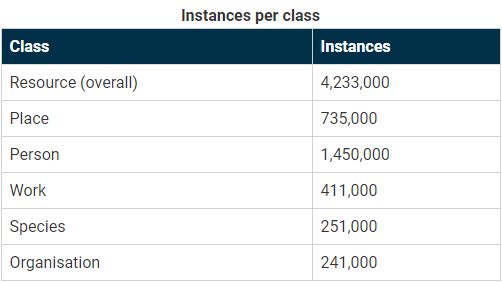
\includegraphics[width=.5\paperwidth]{dbpediaontology}
	\end{center}
	\caption{DBPedia Ontology instances per class \cite{dbpedia2019ontology}}
	\label{fig:ontology}
\end{figure}

The DBpedia extraction framework is responsible for extracting data from Wikipedia into a structured knowledge base, an overview of which is shown in Figure~\ref{fig:extraction}. This extraction is structured into four phases, as described by \citet{lehmann2015dbpedia}:

\begin{itemize}[label={},itemindent=-2em,leftmargin=2em]
	\item {\bf Input:} Wikipedia pages are read from an external source, either from a Wikipedia dump, or using the MediaWiki API.
	\item {\bf Parsing:} Each Wikipedia page is parsed, which transforms the source code of the Wikipedia page into an Abstract Syntax Tree (AST). An AST is a tree representation of the syntactic structure of the source code.
	\item {\bf Extraction:} The Abstract Syntax Tree of each page is forwarded to the extractors. There are many types of extractors, which will later be described, which extract data such as labels, images and infoboxes. Each extractor takes an AST as input and yields a set of Resource Description Framework (RDF) statements. These are XML statements which describe properties and values of resources.
	\item {\bf Output:} These RDF statements are written into sinks, which receive the data.
\end{itemize}

\begin{figure}[h]
	\begin{center}
		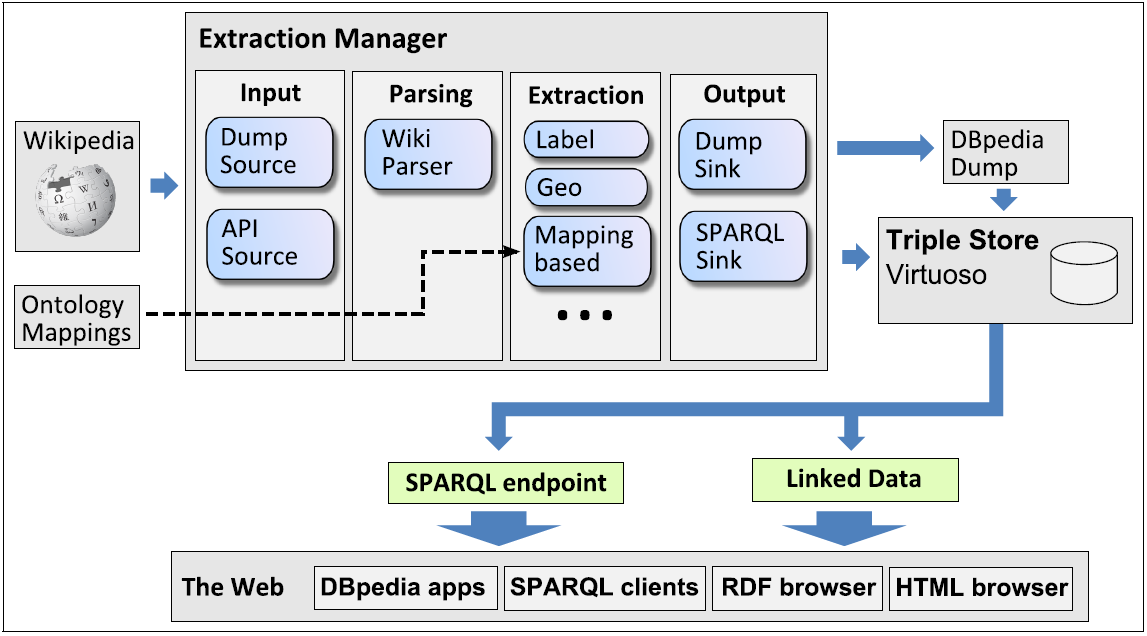
\includegraphics[width=.6\paperwidth]{dbpediaextraction}
	\end{center}
	\caption{DBpedia extraction framework \cite{bizer2009dbpedia}}
	\label{fig:extraction}
\end{figure}

The DBPedia ontology organises its entities using RDF models, each of which has many properties and are linked to subclasses and super-classes. This can be seen in Table~\ref{tab:ontology}, where a subclass may inherit the properties of its parent class. This can assist querying and searching, as we can query the data based on properties of a given class, as well as filtering with conditional queries. 

\begin{table}[h]
	\centering
	\begin{tabular}{{@{}lll@{}}}
		\toprule
		Ontology class & Instances & Example properties \\
		\midrule
		Person & 198,056 & name, birthdate, birthplace, employer, spouse \\
		\hspace{3mm} Artist & 54,262 & activeyears, awards, occupation, genre \\
		\hspace{6mm} Actor & 26,009 & academyaward, goldenglobeaward, activeyears \\
		\hspace{6mm} MusicalArtist & 19,535 & genre, instrument, label, voiceType, activeyears \\

		Athlete & 74,832 & currentTeam, currentPosition, currentNumber \\

		Politician & 12,874 & predecessor, successor, party \\
		\bottomrule
	\end{tabular}
	\caption{Example DBPedia classes and example instances \cite{lehmann2015dbpedia}}
	\label{tab:ontology}
\end{table}

The data extracted by the Extraction Manager is mapped to the ontology classes and properties to provide structured RDF statements. This allows instances of classes to be queried using the SPARQL query language \cite{sparql}, which returns data in the RDF format. The role of RDF is to provide semantics and structure to the information \cite{decker2000semantic}, which aligns with Tim Berners-Lee's vision of the next generation of the Web known as the Semantic Web \cite{berners2001semantic}. The DBPedia RDF Data Set is hosted and published using OpenLink Virtuoso, which provides a public SPARQL endpoint for querying the data \cite{lehmann2015dbpedia}; the RDF Dumps are also available to be downloaded in full.

The DBPedia data set is a strong candidate for use in this project because of its large scope and capacity for querying the data. The public SPARQL endpoint will also allow the dataset to be quickly investigated and tested.

\subsection{Other Candidates}
\label{subsec:candidates}
A widely used resource for data science and machine learning is Kaggle \cite{kaggle}, which is an online community that provides public and licensed datasets for use in data science projects and competitions. Previous works have used the resource to develop computer-aided diagnosis (CAD) systems for diagnosing cancers \cite{kuan2017deep}. More relevant to this project, \citet{uchendu2019characterizing} used the rDany dataset \cite{rdany} to distinguish between human and computer-generated messages. The Kaggle community is therefore a resource worth utilising for this project, and can provide data for further developments to the project in the future.

In the context of Wikipedia information, MediaWiki provides an API for retrieving and searching Wikipedia pages \cite{mediawiki}. While utilising this API would provide full access to the Wikipedia knowledge base, the data is not as manageable or queryable as that provided by the DBPedia resource. An example query response can be seen in Appendix~\ref{app:mediawiki}.

\newpage
\section{Programming Languages}
\label{sec:langreview}
At its core, the language used to implement a chatbot has few criteria; it needs to be able to process natural language, provide a user interface for input and output, and can optionally interact with a data source. A bare minimum chatbot could therefore be implemented with virtually any programming language. However, it is important to consider the capabilities of the language, including support for machine learning, database interactions, and user interface design. This section will compare programming technologies based on their performance, their compatibility with the chatbot models previously discussed in the report, and the availability of libraries and functionality which may be useful for implementing a fully-featured, extensible chatbot.
 
\subsection{Python}
Python has been widely adopted in the scientific industry \cite{bird2009natural}, touted for its extensive collection of scientific libraries \cite{koepke2011python}; it recently eclipsed Java to become the most popular language, according to IEEE Spectrum \cite{cass2019}. Natural language processing can be quickly implemented with libraries such as Natural Language Toolkit (NLTK) \cite{nltk2019}; artificial neural networks (ANNs) can be leveraged with many libraries, including Scikit-learn \cite{pedregosa2011scikit}. Newer developments in machine learning include TensorFlow \cite{abadi2016tensorflow}, which provides a novel learning framework utilised in large-scale machine learning applications such as healthcare \cite{polzin2019} and Google’s own search engine \cite{pichai2015}. In the context of chatbots, Python allows for interpretation of AIML with the python-aiml library \cite{villegas2019}; more comprehensive chatbot libraries can also be utilised, such as ChatterBot \cite{cox2019}. Using Python would therefore provide the freedom to explore various technologies for implementing the project and extend the functionality in the future, given the abundance of relevant libraries.

In terms of linking data sources, the database access layer in Python is inherently weaker than other technologies such as JDBC and ODBC \cite{vermuelen2019}. However, this is mainly a concern for enterprise solutions, as Python’s DB-API specification can connect to most databases \cite{python2017db}. Furthermore, connecting to a SPARQL endpoint and parsing RDF graphs is possible through RDFLib \cite{rdf2019}. Many Python web frameworks can handle user interaction, routing, and security. Some of the popular web frameworks include Django, TurboGears, and Flask \cite{python2020web}. These frameworks vary in their features, but for the scope of this project, it is safe to assume that any of them will fit the criteria and they can be explored further in the experimentation phase.

Python has been used extensively in the machine learning field, and can be seen in many Machine Learning as a Service (MLaas) services; the Microsoft Azure Machine Learning service uses Python for training and modelling \cite{microsoft2019architecture}. Python would be an effective language to use to implement a project of this scope.

\subsection{Java}
Java is widely used in machine learning implementations \cite{witten2005practical, abeel2009java}, and is prevalent in research and enterprise solutions. Many libraries exist to implement machine learning frameworks \cite{kovalev2016deep}, natural language processing \cite{nltk2019}, and AIML interpreters \cite{alice2013}. Java has the advantage of being natively cross-platform since the Java program is compiled into byte-code to be interpreted by the Java virtual machine (JVM) \cite{witten2005practical}; this may beneficial to this project if it is deployed to a Linux web server.

Querying and interpreting RDF data can be achieved using Apache Jena \cite{apachejena}, and dependency management can be facilitated using several tools such as Apache Maven \cite{apachemaven} and Gradle \cite{gradle}. Many web frameworks exist in order to manage web requests, such as Spring \cite{springmanual} and JavaServer Faces \cite{mcclanahan2004javaserver}. Java has been established as being performant and scalable in general-use programming \cite{moreira2000java}, and the JVM is leveraged by other languages such as Scala \cite{odersky2008programming}. Therefore, implementing the project using Java would provide access to a vast array of libraries and frameworks, and allow for further expansion in the future.

\subsection{Alternatives}
Given the diverse landscape of programming languages available, it is worthwhile to consider how related works are implemented. The original implementation of ALICE by \citet{wallace2009anatomy} was originally programmed in Lisp \cite{winston1986lisp}. Since then, Clojure, a Lisp 'dialect' that runs in the JVM \cite{hickey2008clojure}, has been widely used in machine learning \cite{wali2014clojure}, and can easily take advantage of concurrency in multicore and distributed systems \cite{emerick2012clojure}. Similarly, Scala, another JVM language used in data-driven programming \cite{wampler2014programming}, is employed by the DBPedia Lookup project for searching and ranking DBPedia resources by keyword \cite{dbpedialookup}.

Ruby on Rails (RoR) is a web application framework used widely on the Web \cite{paplauskaite2016}. Web applications using this framework benefit from the RoR principles of 'Convention over Configuration' CoC and 'Don't Repeat Yourself' \cite{bachle2007ruby}, which accelerate development of applications. This framework was used effectively by \citet{horzyk2009intelligent} to create a chatbot shop-assistant that adapts to a customer's perceived personality.

\subsection{Conclusion}
Having explored a number of programming languages, it is evident that a project of this scope could be implemented in any of the languages explored above, and many more, due to the availability of relevant libraries. The choice of programming language used for the project will be further explored and justified in Section~\ref{sec:lang}.

\cleardoublepage
\section{Existing Solutions}
\label{sec:existing}
Dialogue systems are abundant in business and consumer use, from ordering pizza with a Google Home device \cite{google2018dominos}, to diagnosing and managing patients’ medical conditions \cite{yourmd2017}. This section will explore existing solutions that are relevant to the scope of this project, as well as broader chat systems currently in use.

\subsection{Google Assistant}
Google Assistant is a popular and highly available intelligent virtual assistant (IVA) offering from Google \cite{lopez2017alexa}. It provides a vast array of functions, such as searching and integration with enabled `smart devices' \cite{googleassistant}. Google Assistant also incorporates other Google services, including search, which facilitates keyword queries about almost any topic \cite{michaely2017keyword}, as seen in Figure~\ref{fig:assistant}.

One standout feature of Google Assistant is its contextual understanding, which Google brands as Continued Conversation \cite{paplauskaite2016}. As concluded by \citet{tulshan2019survey}, Google Assistant is the most effective IVA at contextual understanding, which is demonstrated in Figure~\ref{fig:assistant}.

It is clear that the functionality of Google Assistant eclipses the scope of this project. However, there are several features from which this project can draw inspiration. For example, contextual understanding would be an effective feature to integrate into the chatbot to make conversational queries more efficient. The drawback of Google Assistant is its propietary nature, meaning that we cannot investigate how it is implemented, nor can we extend it in this project.

\begin{figure}[h]
	\centering
    \subfloat[Querying Google Assistant]{{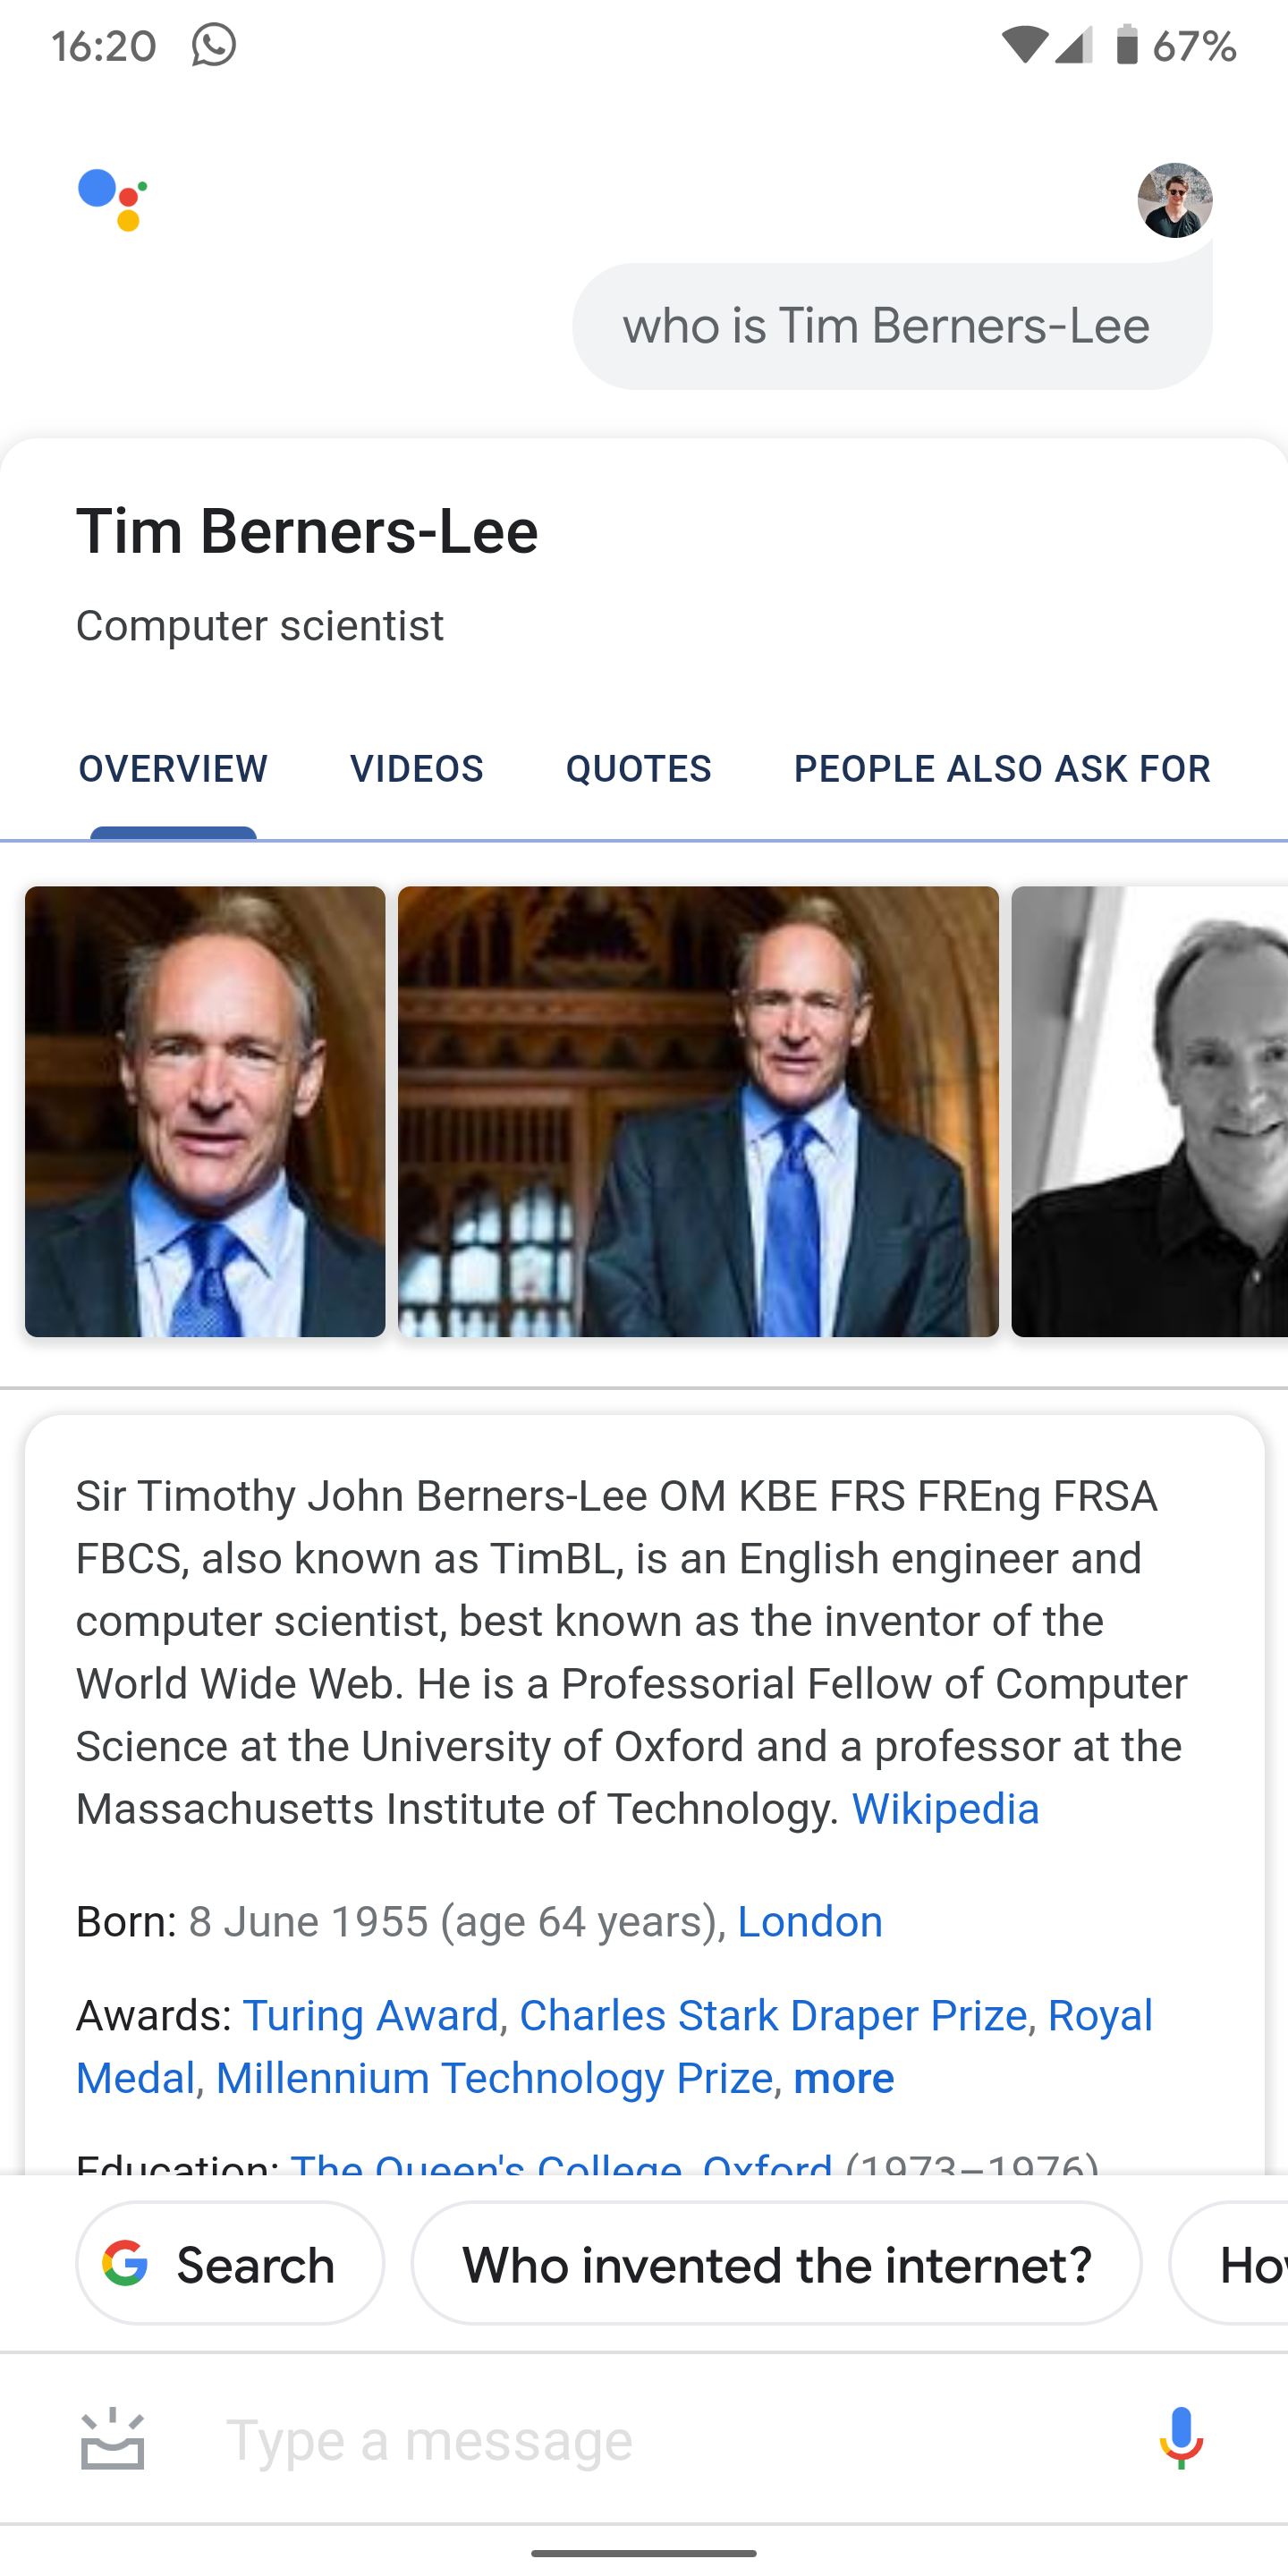
\includegraphics[width=5cm]{assistant1} }}%
    \qquad
	\subfloat[Google Assistant's Continued Conversation]{{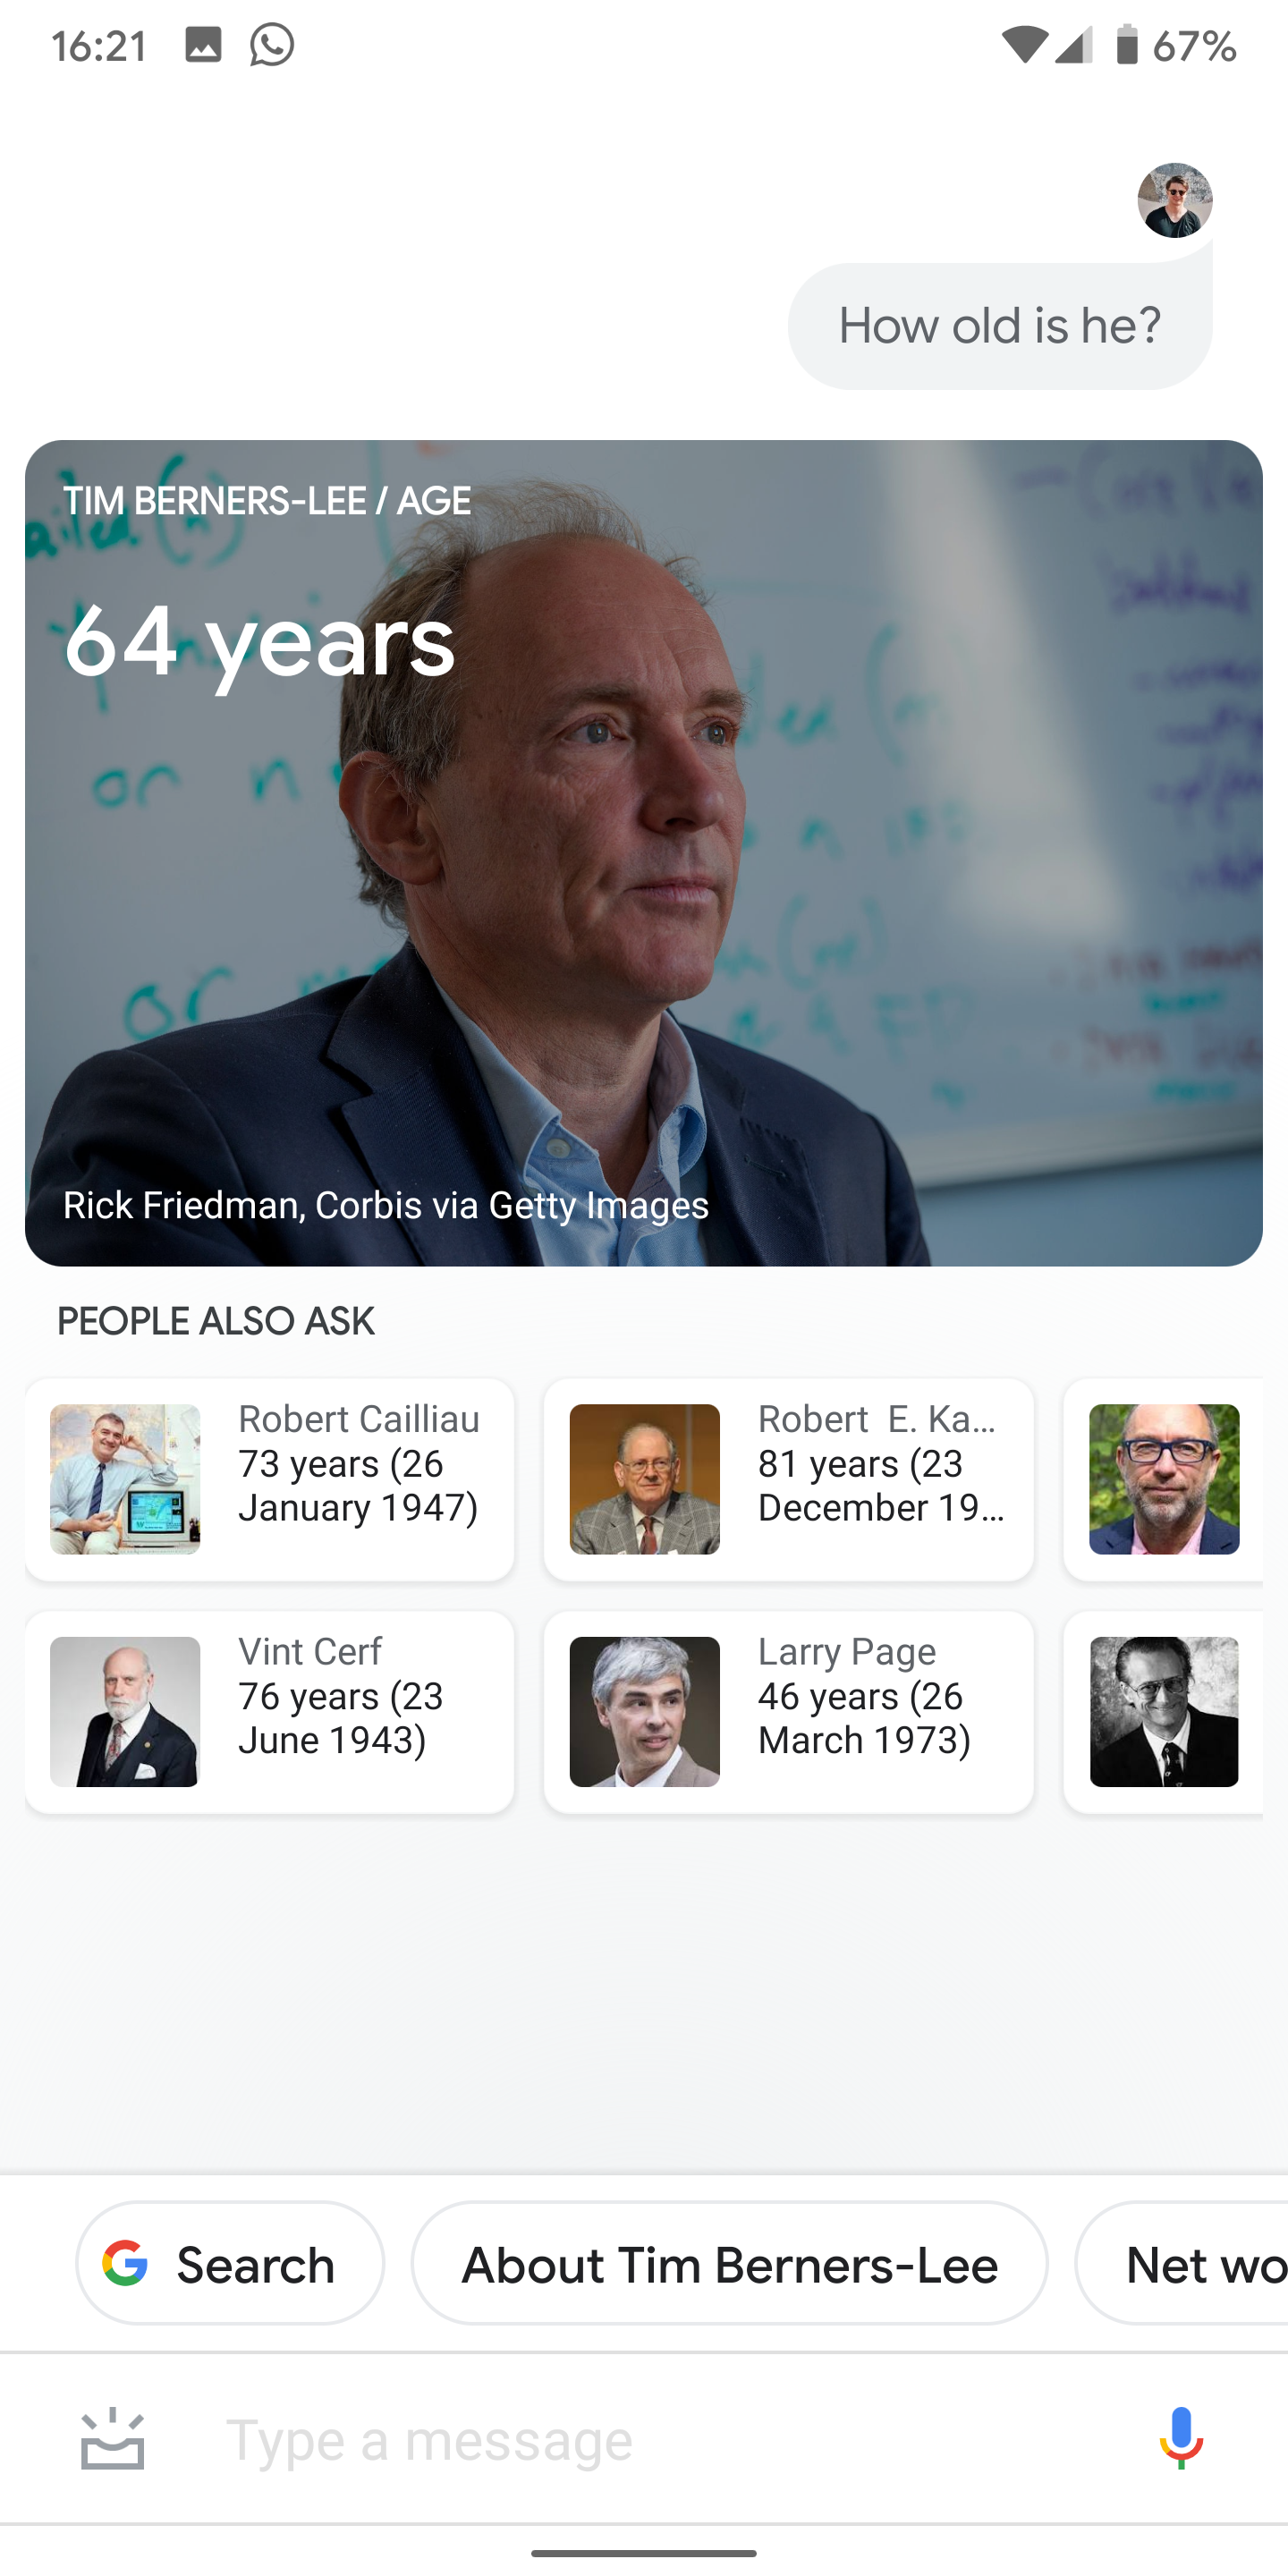
\includegraphics[width=5cm]{assistant2} }}%	
	\caption{A conversation with Google Assistant}
	\label{fig:assistant}
\end{figure}

\newpage
\subsection{DBPedia Chatbot}
\label{sec:dbchatbot}
The system that resembles the scope of this project closest is DBPedia Chatbot \cite{ramngongausbeck2018}. The project integrates with the DBPedia dataset to provide a chatbot which allows users to pose questions, and the system then generates a response using information from the dataset.

Upon investigating the solution, the chatbot can only interpret a small set of predetermined queries. When a query outside of this question set is posed, the chatbot throws an error -- as shown in Figure~\ref{fig:dbchatbot}. This could either be a limitation of the implementation itself, or the publicly available demo website \footnote{http://chat.dbpedia.org/}. Therefore, this project can expand beyond the scope of the implementation provided by \citet{ramngongausbeck2018}, including more advanced queries and filtering. The rich response elements seen in Figure~\ref{fig:dbchatbot} are effective and this project can draw inspiration from them in the final implementation.

\begin{figure}[h]
	\centering
	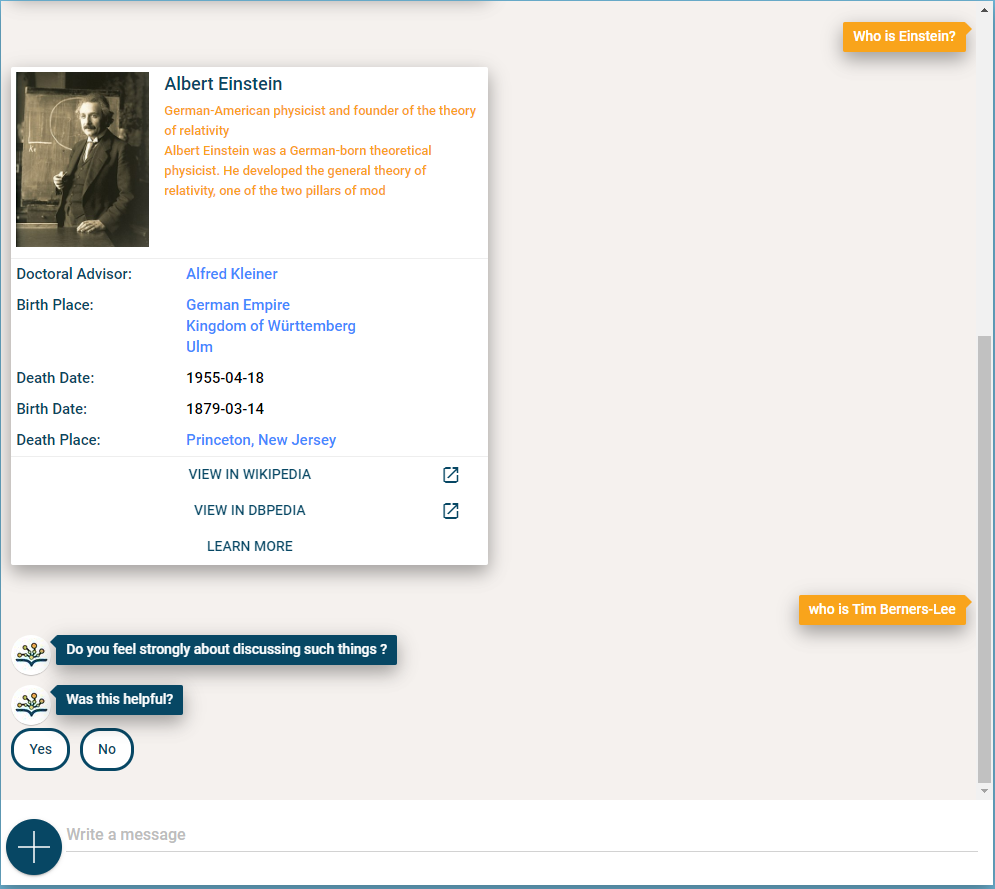
\includegraphics[width=.5\paperwidth]{dbchatbot}
	\caption{DBPedia Chatbot implementation \cite{ramngongausbeck2018}}
	\label{fig:dbchatbot}
\end{figure}

\newpage
\subsection{Mitsuku}
\label{subsec:Mitsuku}
Mitsuku is a chatbot implementation created by Steve Worswick \cite{worswick2018mitsuku} which has won the Loebner Prize a record five times \cite{aisb2019}. The chatbot is implemented using AIML \cite{higashinaka2014towards}, and is designed to handle open conversation with Mitsuku, who claims to be an eighteen year-old girl \cite{abdul2015survey}.

Mitsuku deals well with general conversation and banter, and responds in a humourous and intelligent manner. As can be seen in my dialogue with her in Appendix~\ref{app:mitsuku}, this implementation is effective at establishing a distinct and discernible personality for Mitsuku. Although Mitsuku only seems to handle a set of predetermined queries (see Figure~\ref{fig:mitsuku}), it is clear that the purpose of Mitsuku is not to serve as a knowledge base, but as a general-purpose conversational bot. She handles open questions intelligently, and seems to have a large repository of conversation topics and responses. She also manages multi-turn dialogues well, and is effective at maintaining the context of the conversation. Mitsuku is closed-source, so the AIML definitions cannot be explored, but this project can take inspiration from the conversation style of Mitsuku.

\begin{figure}[h]
	\centering
	\subfloat[Querying Mitsuku]{{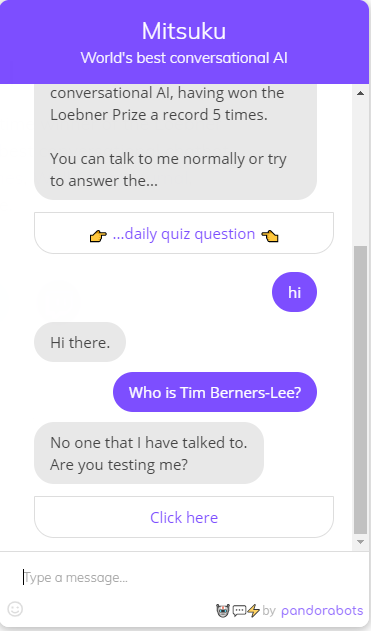
\includegraphics[width=5cm]{mitsuku1} }}%
	\qquad
	\subfloat[Mitsuku known result]{{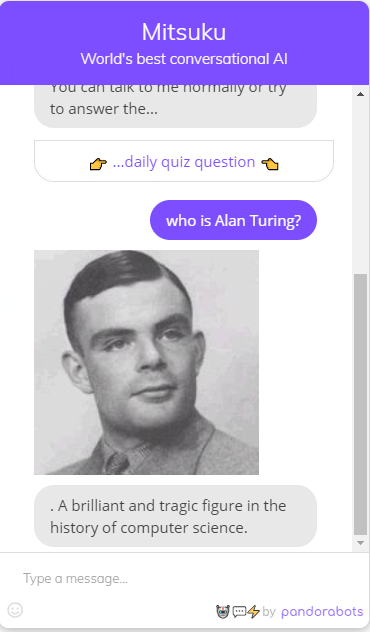
\includegraphics[width=5cm]{mitsuku2} }}%	
	\caption{A conversation with Mitsuku}
	\label{fig:mitsuku}
\end{figure}

%\subsection{DBPedia Spotlight}

\newpage
\section{Related Work}
Chatbot designs have been thoroughly investigated by \citet{abdul2015survey}, who conclude that there does not yet exist a common chatbot approach, although pattern matching techniques such as AIML are effective in closed-domain systems. It is, however, a field that is seeing frequent and significant developments from researchers and companies.

\citet{yan2016learning} found that a neural network approach, known as {\it deep learning-to-respond}, outperforms pattern-matching and retrieval-based models in open-domain generative systems. Similarly, \citet{mikolov2011extensions} concludes that recurrent neural network language models are the most effective technique in linguistic tasks such as machine translation and automatic speech recognition.

As examined in Section~\ref{sec:dbchatbot}, \citet{ramngongausbeck2018} implemented a chatbot using DBPedia as a datasource. This work can be extended in the scope of this project, by providing a complete and more advanced system. \citet{bradevsko2012survey} observed a trend in chatbot systems towards {\it semantics}, which will be further explored in this project.

\section{Conclusion}
This review has explored chatbots and how they are currently being used in industry and research. We are seeing a trend towards chatbots being used in many businesses, from customer service to healthcare; the fields of human-computer interaction and machine learning are seeing many new and significant developments. Chatbot systems are becoming prevalent in modern life, so exploring this evolution will be one of the main objectives of this project.

As the Web trends towards the new era of the Semantic Web, methods of extracting and interpreting information are evolving. Developing a chatbot to understand semantic data will form a basis for future developments and extensions of this project.

The next step for this project is to design a chatbot solution based on the outcome of the research. As is evident from the existing solutions that have been explored, a chatbot can be implemented with an array of available technologies. The next sections of this report will consider how these technologies can be implemented to develop a novel and successful chatbot solution that fits the requirements determined in the analysis phase.





